\documentclass[11pt,a4paper]{article}

\usepackage[T1]{fontenc}
\usepackage{lmodern}
\usepackage[margin=2.4cm]{geometry}
\usepackage{amsmath}
\usepackage{graphicx}
\usepackage{booktabs}
\usepackage{xcolor}
\usepackage{microtype}
\usepackage[colorlinks=true,linkcolor=accent,urlcolor=accent]{hyperref}
\usepackage{tcolorbox}
\usepackage{titlesec}
\usepackage{float}
\usepackage{parskip}

\definecolor{accent}{HTML}{2a78d6}
\definecolor{warm}{HTML}{eb6834}
\definecolor{ink}{HTML}{1a1a19}
\definecolor{ink2}{HTML}{52514e}
\definecolor{rule}{HTML}{dedcd6}
\definecolor{panel}{HTML}{f4f3f0}

\color{ink}
\titleformat{\section}{\normalfont\large\bfseries\color{ink}}{\thesection.}{0.6em}{}
\titleformat{\subsection}{\normalfont\normalsize\bfseries\color{ink}}{}{0em}{}
\titlespacing*{\section}{0pt}{1.5em}{0.5em}

\newcommand{\code}[1]{{\ttfamily\small #1}}

\begin{document}

\begin{center}
{\LARGE\bfseries Two errors in the network model's\\[2pt] load and PV equations\par}
\vspace{0.7em}
{\large\color{ink2} What they were, why nobody saw them,\\ and what they change\par}
\vspace{0.9em}
{\color{ink2}\small Tulio Coura \quad$\cdot$\quad 26 August 2026 \quad$\cdot$\quad all nine transformers\par}
\end{center}

\vspace{0.6em}

\begin{tcolorbox}[colback=panel,colframe=rule,boxrule=0.7pt,arc=2pt,
                  left=10pt,right=10pt,top=9pt,bottom=9pt]
\textbf{The short version.} The model contained two mistakes in the equations that
describe how much current a house draws when its voltage changes. Both had been there
since the beginning. Both are now fixed, and every transformer has been re-run.

\medskip
The effect is stranger than you might expect. The flexibility region does not grow or
shrink so much as \emph{turn}: it reaches further into reactive import and less far into
export, by up to 33.7~kW. That rotation appears on \textbf{all nine transformers}, in the
same direction, which is what you would predict from the specific terms that were wrong.

\medskip
Where the battery schedule is unchanged, the region's \emph{area} moves by a median of
0.05\%. Where the fix also moved the schedule, it moves by up to 7\%. So conclusions about
\emph{how much} flexibility a feeder has are safe; conclusions about \emph{specific
operating points}, especially reactive ones, are the ones to re-examine.
\end{tcolorbox}

\section{What these equations are for}

The physics of a power network is nonlinear. A house that draws a fixed amount of power
draws \emph{more current} when its voltage sags, and less when it rises. That
relationship is a division, not a multiplication, and an optimiser cannot work with it
directly.

So the model does what engineers always do with an awkward curve: it replaces it with a
straight line. It picks a starting voltage --- here, the flat-start value where every
bus sits at its nominal voltage --- and asks a simple question at that point:

\begin{center}
\itshape if the voltage moves a little, how much does the current move?
\end{center}

The answer is a set of slopes. There are eight of them: one for each combination of
\{real, imaginary\} current against \{real, imaginary\} voltage, for loads and for PV.
They are ordinary partial derivatives, worked out once by hand and typed into the model
as formulas.

\textbf{Two of those eight were wrong.} Not the physics around them --- the network
equations, the limits, the battery model are all sound. Just two of the eight slopes.

\section{The first error: a parenthesis in the wrong place}

The imaginary part of a load's current is
\[
  I_{\mathrm{im}} \;=\; \frac{P_0 V_{\mathrm{im}} - Q_0 V_{\mathrm{re}}}
                              {V_{\mathrm{re}}^2 + V_{\mathrm{im}}^2}.
\]

Differentiating with respect to $V_{\mathrm{im}}$ gives two terms --- one carrying the
active power $P_0$, one carrying the reactive power $Q_0$:
\[
  \frac{\partial I_{\mathrm{im}}}{\partial V_{\mathrm{im}}}
  \;=\;
  \frac{\;P_0\!\left(V_{\mathrm{re}}^2 - V_{\mathrm{im}}^2\right)
        \;+\; 2\,Q_0 V_{\mathrm{re}} V_{\mathrm{im}}\;}
       {\left(V_{\mathrm{re}}^2 + V_{\mathrm{im}}^2\right)^2}.
\]

In the model, the closing bracket sat one term too late, so the $Q_0$ term ended up
\emph{inside} the multiplication by $P_0$:

\begin{center}
\begin{tabular}{@{}ll@{}}
\toprule
\textbf{was} & \code{P0*( Vre0\^{}2 - Vim0\^{}2 + 2*Q0*Vre0*Vim0 ) / (.)\^{}2} \\
\textbf{now} & \code{( P0*(Vre0\^{}2 - Vim0\^{}2) + 2*Q0*Vre0*Vim0 ) / (.)\^{}2} \\
\bottomrule
\end{tabular}
\end{center}

\subsection{Why this is worse than a typo}

You might expect a stray bracket to distort a term. This one removed it.

Everything inside the model is in per unit on a 1~MW base. A one-kilowatt household load
is therefore $0.001$. Multiplying the reactive term by $P_0$ did not tilt it --- it
shrank it by a factor of about a thousand.

In practice, the reactive coupling in that equation was simply \textbf{missing}.

\section{The second error: the wrong quantity}

The real part of a PV system's current is
\[
  I_{\mathrm{re}}^{\mathrm{PV}} \;=\; \frac{G V_{\mathrm{re}}}
                                            {V_{\mathrm{re}}^2 + V_{\mathrm{im}}^2},
  \qquad\text{so}\qquad
  \frac{\partial I_{\mathrm{re}}^{\mathrm{PV}}}{\partial V_{\mathrm{im}}}
  \;=\; \frac{-2\,G\,V_{\mathrm{re}} V_{\mathrm{im}}}
             {\left(V_{\mathrm{re}}^2 + V_{\mathrm{im}}^2\right)^2},
\]
where $G$ is the PV output. The model used \emph{net} demand --- the house load minus its
PV, \code{P0minGenP} --- where it should have used the PV output alone:

\begin{center}
\begin{tabular}{@{}ll@{}}
\toprule
\textbf{was} & \code{( -2*P0minGenP(d,t)*Vre0*Vim0 ) / (.)\^{}2} \\
\textbf{now} & \code{( -2*GenP0(d,t)*Vre0*Vim0 ) / (.)\^{}2} \\
\bottomrule
\end{tabular}
\end{center}

Every other PV slope in the model uses the PV output. The current being differentiated is
defined from the PV output. Only this one line disagreed.

\subsection{Why this one changes sign with the sun}

Write out what the model used against what it should have used, in per unit:

\begin{center}
\begin{tabular}{@{}lrrl@{}}
\toprule
\textbf{Time of day} & \textbf{used} & \textbf{correct} & \textbf{effect} \\
\midrule
Midday, PV 3\,kW, load 1\,kW      & $-0.0020$ & $+0.0030$ & {\color{warm}\bfseries sign flipped} \\
Dawn or dusk, PV 0.5\,kW, load 1\,kW & $+0.0005$ & $+0.0005$ & accidentally right \\
Night, PV 0\,kW, load 1\,kW       & $+0.0010$ & $0$       & invented from nothing \\
\bottomrule
\end{tabular}
\end{center}

At midday, when PV dominates the house load, the term pointed \textbf{the wrong way}. At
dawn and dusk, where load and PV happen to be similar, subtracting one from the other
lands close to the right answer by luck. At night it produced a PV sensitivity for a
panel generating nothing.

This is a testable prediction: the damage should be worst around noon and near zero at
either end of the day. That is exactly what the measurement shows.

\subsection{A check that the fix is right}

After correction, this slope is character-for-character identical to another one in the
model that was always correct --- the one for imaginary current against real voltage.

That is not a coincidence and not a copy-and-paste. For PV, the two cross-slopes are
mathematically the same quantity:
\[
  \frac{\partial I_{\mathrm{re}}}{\partial V_{\mathrm{im}}}
  \;=\;
  \frac{\partial I_{\mathrm{im}}}{\partial V_{\mathrm{re}}}
  \;=\;
  \frac{-2\,G\,V_{\mathrm{re}} V_{\mathrm{im}}}
       {\left(V_{\mathrm{re}}^2 + V_{\mathrm{im}}^2\right)^2}.
\]

The corrected line landed on a value the model already contained, independently, in
another place. The remaining six slopes were re-derived by hand and are all correct.

\section{Why nobody saw them}

This is the uncomfortable part: \textbf{neither error makes anything fail.}

These slopes are not constraints. Nothing can violate them. They do not affect whether a
solution exists, and they do not change what the solver reports. Both the old and the new
model return \emph{Optimal} on all 5{,}184 problems --- 576 on each of the nine
transformers --- report healthy voltages, and pass every after-the-fact physical check we
have: no voltage violations, in either version, anywhere.

The only symptom is a slightly wrong sensitivity, which flows quietly into the power
balance and out into the results.

There was nothing to notice. The errors were found by re-deriving all eight slopes from
scratch during a full read of the model --- not by chasing a bad number.

\section{What was measured}

Every transformer was run twice, before and after the fix, with everything else held
identical: the per-transformer reduced network, the exact formulation, 48 half-hours,
12 directions each. Nine transformers, 5{,}184 boundary points per pass.

\begin{center}
\begin{tabular}{@{}lr@{}}
\toprule
Solve status & 576 of 576 optimal, every transformer, both passes \\
Directions that changed & \textbf{5{,}180 of 5{,}184} \\
Largest boundary movement & \textbf{33.7 kW} (TR5) \\
Typical boundary movement & 1.8 kW \\
Voltage violations introduced & none, on any transformer \\
Change in runtime & negligible \\
\bottomrule
\end{tabular}
\end{center}

Nearly every direction moved. Yet the area barely did. Those two facts only fit together
one way: the region is \textbf{rotating}, not growing or shrinking.

\begin{center}
\begin{tabular}{@{}lr@{}lr@{}}
\toprule
\multicolumn{2}{@{}l}{\textbf{Reactive-import side}} & \multicolumn{2}{l}{\textbf{Export side}} \\
\midrule
\phantom{00}60\textdegree & $+3.5$ kW & \quad 180\textdegree & $-2.9$ kW \\
\phantom{00}90\textdegree & $+3.6$ kW & \quad 210\textdegree & $-3.5$ kW \\
120\textdegree & $+1.5$ kW & \quad 240\textdegree & $-2.3$ kW \\
\bottomrule
\end{tabular}
\end{center}

One side pushes out, the other pulls in, by matching amounts. The area survives because
the two cancel.

\textbf{And this is not one transformer's quirk.} All nine push out on the reactive-import
side and pull in on the export side --- nine out of nine, same sign, same shape. That is
the strongest evidence that what is being seen is the correction doing what the algebra
says it should, rather than numerical noise.

This is what you would predict from the two errors. Both are \emph{cross} terms --- they
link the real and imaginary parts of the electrical quantities, which is another way of
saying they govern the interaction between active and reactive power. Correcting them
moves reactive power. It is not random error; it is a systematic shift along one axis, and
it does not average out.

\begin{figure}[H]
\centering
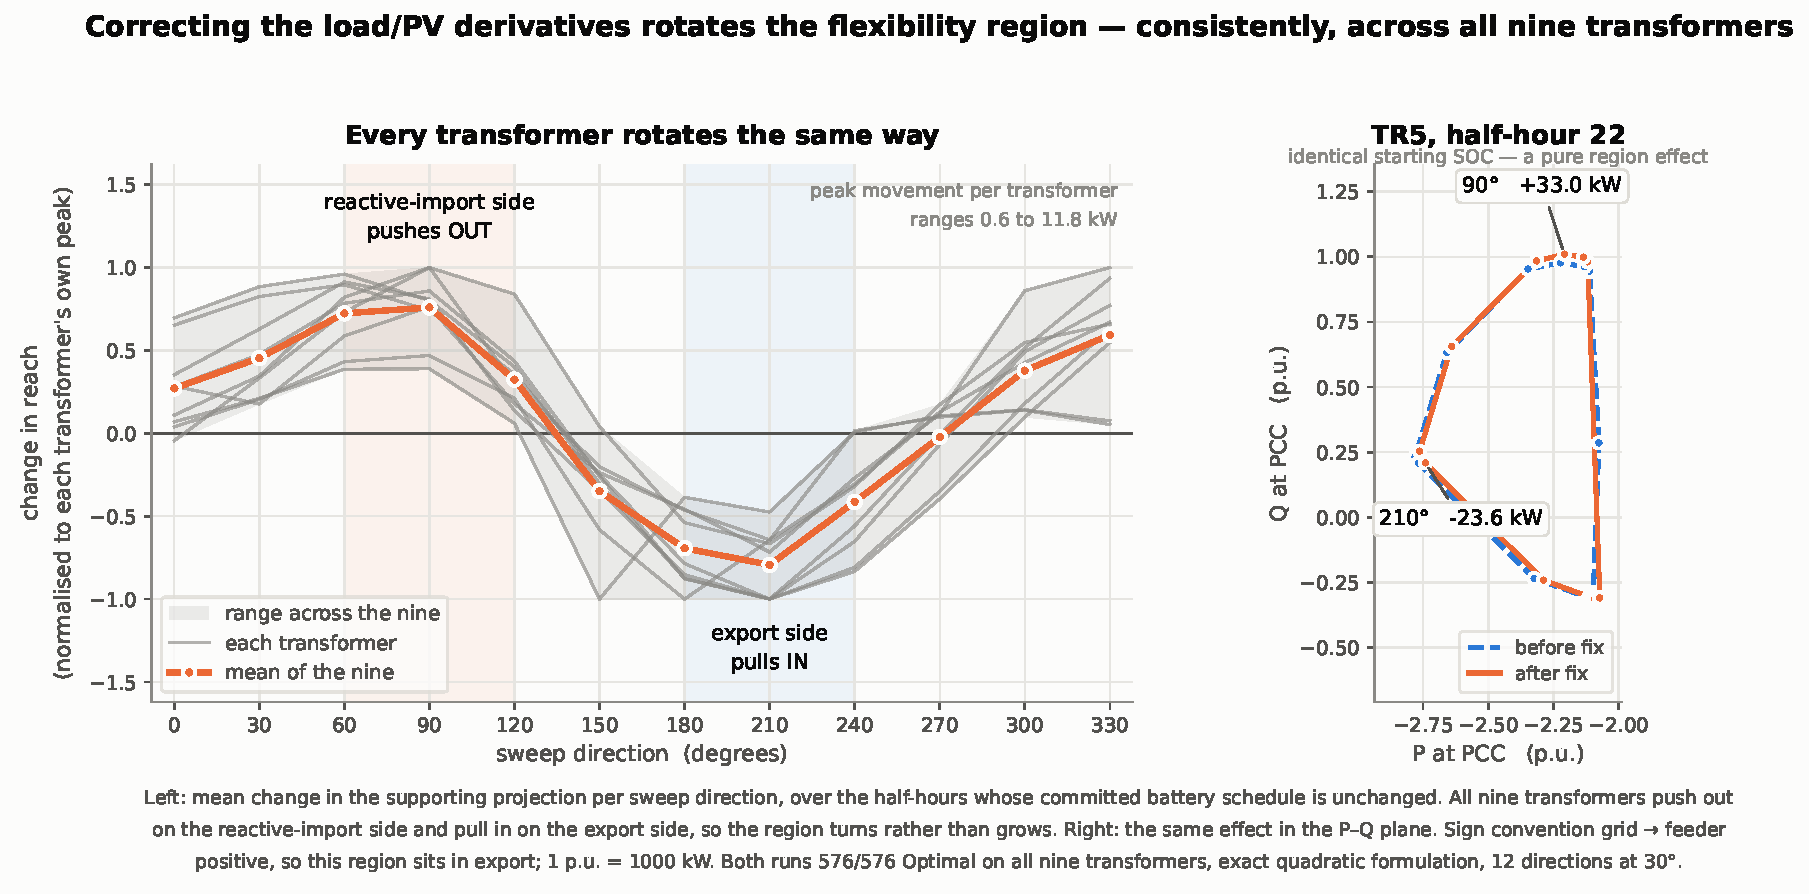
\includegraphics[width=\textwidth]{derivfix_summary.pdf}
\caption{Left: the change in reach by sweep direction, one grey line per transformer,
each normalised to its own peak so the shapes can be compared. Every one of the nine
pushes out on the reactive-import side and pulls in on the export side. Right: the same
effect in the P--Q plane, on a half-hour where the battery schedule is unchanged, so the
movement is the region and nothing else. The right-hand edge, where active power sets the
limit, hardly moves.}
\end{figure}

\subsection{One honest caveat}

The battery schedule also changed.

The model decides what the batteries actually do using the same equations, so correcting
them moved that decision too. In those half-hours the difference between the two runs
mixes two things: the region moving, and the batteries starting somewhere else. Splitting
them apart matters, because the two give very different numbers:

\begin{center}
\begin{tabular}{@{}lrrr@{}}
\toprule
Half-hours & count & median area change & worst \\
\midrule
Battery schedule unchanged & 151 & $-0.05\%$ & $-2.8\%$ \\
Battery schedule also moved & 281 & $-0.26\%$ & $\mathbf{-7.1\%}$ \\
\bottomrule
\end{tabular}
\end{center}

So the region on its own is stable --- 146 of the 151 clean half-hours move by less than
1\%. The large swings live where the fix also rescheduled the batteries.

Neither number is wrong. The new schedule is the correct one; the old was produced by the
faulty equations. But it does mean the published battery trajectories are affected too,
not only the regions.

That rescheduling is narrow. On the worst transformer it touches \textbf{3 batteries out
of 77}, in the midday window, and the worst of them charges to a full state of charge
where the old model left it at 60\%. By the end of the day 75 of those 77 batteries are
back to identical. The fix restores the PV coupling term that was sign-flipped at exactly
those hours, so midday is precisely where one would expect it to bite.

\section{What this means}

\begin{tcolorbox}[colback=panel,colframe=rule,boxrule=0.7pt,arc=2pt,
                  left=10pt,right=10pt,top=9pt,bottom=9pt]
\textbf{If a conclusion is about how much flexibility a feeder can offer,} it stands.
Where the battery schedule is unchanged the area moves by a median of 0.05\%, and 146 of
151 such half-hours move by less than 1\%.

\textbf{If a conclusion is about a specific operating point} --- a stated maximum import
or export at a given hour --- it moves by up to 33.7~kW.

\textbf{If a conclusion is about reactive power,} that is where to look hardest. The error
is systematic on that axis, it points the same way on all nine transformers, and it does
not average out.

\textbf{If a result depends on the battery trajectory} rather than the region, check the
midday window. Seven of the nine transformers reschedule there.
\end{tcolorbox}

The two lines sit in the network physics that the rest of the model was built on. Anything
else that model has been used for carries them too.

\section{What happens next}

The fix is committed and all nine transformers have been re-run and measured. Nothing
further is pending on this correction.

One larger approximation remains untouched. The model draws its straight-line
approximation once, at the flat-start voltage, and never redraws it as the solution moves
away. The gap between the approximation and the true voltage reaches about 1.6\% ---
larger than the error just corrected. Fixing that would mean regenerating everything
again, so it is worth deciding deliberately rather than drifting into it.

\end{document}
